%% Beginning of file 'sample7.tex'
%%
%% Version 7. Created January 2025.  
%%
%% AASTeX v7 calls the following external packages:
%% times, hyperref, ifthen, hyphens, longtable, xcolor, 
%% bookmarks, array, rotating, ulem, and lineno 
%%
%% RevTeX is no longer used in AASTeX v7.
%%
\documentclass[linenumbers,trackchanges]{aastex7}
%%
%% This initial command takes arguments that can be used to easily modify 
%% the output of the compiled manuscript. Any combination of arguments can be 
%% invoked like this:
%%
%% \documentclass[argument1,argument2,argument3,...]{aastex7}
%%
%% Six of the arguments are typestting options. They are:
%%
%%  twocolumn   : two text columns, 10 point font, single spaced article.
%%                This is the most compact and represent the final published
%%                derived PDF copy of the accepted manuscript from the publisher
%%  default     : one text column, 10 point font, single spaced (default).
%%  manuscript  : one text column, 12 point font, double spaced article.
%%  preprint    : one text column, 12 point font, single spaced article.  
%%  preprint2   : two text columns, 12 point font, single spaced article.
%%  modern      : a stylish, single text column, 12 point font, article with
%% 		  wider left and right margins. This uses the Daniel
%% 		  Foreman-Mackey and David Hogg design.
%%
%% Note that you can submit to the AAS Journals in any of these 6 styles.
%%
%% There are other optional arguments one can invoke to allow other stylistic
%% actions. The available options are:
%%
%%   astrosymb    : Loads Astrosymb font and define \astrocommands. 
%%   tighten      : Makes baselineskip slightly smaller, only works with 
%%                  the twocolumn substyle.
%%   times        : uses times font instead of the default.
%%   linenumbers  : turn on linenumbering. Note this is mandatory for AAS
%%                  Journal submissions and revisions.
%%   trackchanges : Shows added text in bold.
%%   longauthor   : Do not use the more compressed footnote style (default) for 
%%                  the author/collaboration/affiliations. Instead print all
%%                  affiliation information after each name. Creates a much 
%%                  longer author list but may be desirable for short 
%%                  author papers.
%% twocolappendix : make 2 column appendix.
%%   anonymous    : Do not show the authors, affiliations, acknowledgments,
%%                  and author contributions for dual anonymous review.
%%  resetfootnote : Reset footnotes to 1 in the body of the manuscript.
%%                  Useful when there are a lot of authors and affiliations
%%		    in the front matter.
%%   longbib      : Print article titles in the references. This option
%% 		    is mandatory for PSJ manuscripts.
%%
%% Since v6, AASTeX has included \hyperref support. While we have built in 
%% specific %% defaults into the classfile you can manually override them 
%% with the \hypersetup command. For example,
%%
%% \hypersetup{linkcolor=red,citecolor=green,filecolor=cyan,urlcolor=magenta}
%%
%% will change the color of the internal links to red, the links to the
%% bibliography to green, the file links to cyan, and the external links to
%% magenta. Additional information on \hyperref options can be found here:
%% https://www.tug.org/applications/hyperref/manual.html#x1-40003
%%
%% The "bookmarks" has been changed to "true" in hyperref
%% to improve the accessibility of the compiled pdf file.
%%
%% If you want to create your own macros, you can do so
%% using \newcommand. Your macros should appear before
%% the \begin{document} command.
%%
\newcommand{\vdag}{(v)^\dagger}
\newcommand\aastex{AAS\TeX}
\newcommand\latex{La\TeX}
%%%%%%%%%%%%%%%%%%%%%%%%%%%%%%%%%%%%%%%%%%%%%%%%%%%%%%%%%%%%%%%%%%%%%%%%%%%%%%%%
%%
%% The following section outlines numerous optional output that
%% can be displayed in the front matter or as running meta-data.
%%
%% Running header information. A short title on odd pages and 
%% short author list on even pages. Note that this
%% information may be modified in production.
%%\shorttitle{AASTeX v7 Sample article}
%%\shortauthors{The Terra Mater collaboration}
%%
%% Include dates for submitted, revised, and accepted.
%%\received{February 1, 2025}
%%\revised{March 1, 2025}
%%\accepted{\today}
%%
%% Indicate AAS Journal the manuscript was submitted to.
%%\submitjournal{PSJ}
%% Note that this command adds "Submitted to " the argument.
%%
%% You can add a light gray and diagonal water-mark to the first page 
%% with this command:
%% \watermark{text}
%% where "text", e.g. DRAFT, is the text to appear.  If the text is 
%% long you can control the water-mark size with:
%% \setwatermarkfontsize{dimension}
%% where dimension is any recognized LaTeX dimension, e.g. pt, in, etc.
%%%%%%%%%%%%%%%%%%%%%%%%%%%%%%%%%%%%%%%%%%%%%%%%%%%%%%%%%%%%%%%%%%%%%%%%%%%%%%%%
%%
%% Use this command to indicate a subdirectory where figures are located.
%%\graphicspath{{./}{figures/}}
%% This is the end of the preamble.  Indicate the beginning of the
%% manuscript itself with \begin{document}.

\begin{document}

\title{A study on Velocity Dispersion in the Milky Way Andromeda Merger}

%% A significant change from AASTeX v6+ is in the author blocks. Now an email
%% address is required for each author. This means that each author requires
%% at least one of the following:
%%
%% \author
%% \affiliation
%% \email
%%
%% If these three commands are not available for each author, the latex
%% compiler will issue an error and if you force the latex compiler to continue,
%% it will generate an incomplete pdf.
%%
%% Multiple \affiliation commands are allowed and authors can also include
%% an optional \altaffiliation to indicate a status, i.e. Hubble Fellow. 
%% while affiliations are indexed as footnotes, altaffiliations are noted with
%% with a non-numeric footnote that is set away from the numeric \affiliation 
%% footnotes. NOTE that if an \altaffiliation command is used it must 
%% come BEFORE the \affiliation call, right after the \author command, in 
%% order to place the footnotes in the proper location. Because non-numeric
%% symbols are used, \altaffiliation should be used sparingly.
%%
%% In v7 the \author command takes an optional argument which provides 
%% additional metadata about the author. Authors can provide the 16 digit 
%% ORCID, the surname (family or last) name, the given (first or fore-) name, 
%% and a name suffix, e.g. "Jr.". The syntax is:
%%
%% \author[orcid=0000-0002-9072-1121,gname=Gregory,sname=Schwarz]{Greg Schwarz}
%%
%% This name metadata in not shown, it is only for parsing by the peer review
%% system so authors can be more easily identified. This name information will
%% also be sent to the publisher so they can include it in the CROSSREF 
%% metadata. Including an orcid will hyperlink the author name to the 
%% author's ORCID page. Note that  during compilation, LaTeX will do some 
%% limited checking of the format of the ID to make sure it is valid. If 
%% the "orcid-ID.png" image file is  present or in the LaTeX pathway, the 
%% ORCID icon will appear next to the authors name.
%%
%% Even though emails are now required for each author, the \email does not
%% produce output in the compiled manuscript unless the optional "show" command
%% is used. For example,
%%
%% \email[show]{greg.schwarz@aas.org}
%%
%% All "shown" emails are show in the bottom left of the first page. Due to
%% space constraints, only a few emails should be shown. 
%%
%% To identify a corresponding author, use the \correspondingauthor command.
%% The command appends "Corresponding Author: " to the argument it appears at
%% the bottom left of the first page like the output from \email. 

\author{Matan Lagnado}
\affiliation{University of Arizona}
\email{mlagnado@arizona.edu}



%% Use the \collaboration command to identify collaborations. This command
%% takes an optional argument that is either a number or the word "all"
%% which tells the compiler how many of the authors above the command to
%% show. For example "\collaboration[all]{(DELVE Collaboration)}" wil include
%% all the authors above this command.
%%
%% Mark off the abstract in the ``abstract'' environment. 

%% Keywords should appear after the \end{abstract} command. 
%% The AAS Journals now uses Unified Astronomy Thesaurus (UAT) concepts:
%% https://astrothesaurus.org
%% You will be asked to selected these concepts during the submission process
%% but this old "keyword" functionality is maintained in case authors want
%% to include these concepts in their preprints.
%%
%% You can use the \uat command to link your UAT concepts back its source.

%% From the front matter, we move on to the body of the paper.
%% Sections are demarcated by \section and \subsection, respectively.
%% Observe the use of the LaTeX \label
%% command after the \subsection to give a symbolic KEY to the
%% subsection for cross-referencing in a \ref command.
%% You can use LaTeX's \ref and \label commands to keep track of
%% cross-references to sections, equations, tables, and figures.
%% That way, if you change the order of any elements, LaTeX will
%% automatically renumber them.

\section{Introduction} 

How does velocity dispersion change through the interaction/collision between MW and M31? In the interaction between the two masses there are many stars interacting with each other causing changes in trajectories as well as velocity. After the two galaxies collide the velocity dispersion will be important to predict the outcome. 'Heating' in a galaxy refers to the chaotic movement of stars, just like gas in a box that moves more randomly when it is being heated. A greater dispersion of vertical velocity, in and out of the plane of the galaxy, refers to more heating. We would expect the vertical velocity dispersion to change dramatically during the collision because of forces acting on the stars that change direction very rapidly. By calculating the ratio of  $\frac{V_{rot}}{\sigma}$ at each time step we can get an understanding of how rotational velocities and their dispersion change during the collision.

Understanding how the velocity distribution changes throughout the collision helps us understand how galaxies evolve when they interact with their neighbors. Various forces influences the velocity dispersion which describes the changes in the shape of a galaxy. A better understanding  can help us understand what influences changes in vertical velocity dispersions (thickening of the galactic plane).

When a galaxy merges with another galaxy the large disturbance in each of their systems causes star's movements to change. The velocity dispersion is a way to measure the average movement of stars through a galaxy. Just as when we look at water we may not see the intricate movement of each water molecule but we can clearly tell which direction a river flows. Continuing this analogy if another river's water is diverted and connects with another river the flow rate may change abruptly with water swirling around trying to find an optimal path. When two galaxies merge there are forces that drastically change speeds and flow of where stars are moving but with each close approach of each galaxy the stars begin to settle and find equilibrium as seen in figure 1 \cite{Stickley_2012}. These changes can have an effect on the overall structure of the galaxy as well, for example a high vertical velocity dispersion is supports a thickened disk model \cite{Dalcanton_2023}.

\begin{figure}[h]
    \centering
    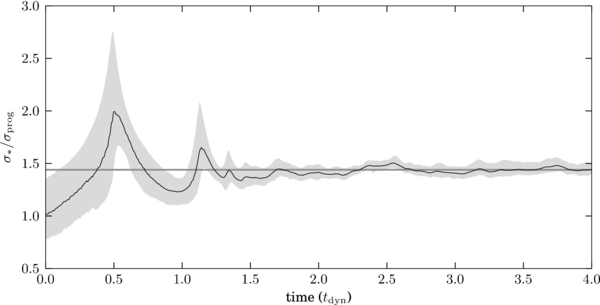
\includegraphics[width=0.75\linewidth]{Stickley2012.jpg}
    \caption{Shows how velocity dispersion changes throughout a merger. Black line is the mean, with uncertainty within the shaded gray region. The gray line is the final mean value of the dispersion.\cite{Stickley_2012}}
    \label{fig:enter-label}
\end{figure}

Many questions on this topic relate to creating more accurate and higher resolution models to describe and predict velocity dispersion in galaxies \cite{Han_2024}. To create more accurate models more data is required which will come with the completion of the Vera C. Rubin Observatory \cite{refId0}. Following more accurate models higher resolution models can be constructed to consider details such as dust absorption as well as 3D velocity dispersions \cite{Han_2024}. 


\section{Proposal}

How does the velocity dispersion of each galaxy(MW/M31) evolve throughout the interaction? How can the velocity dispersion be compared to the present day(pre-collision)?

The most important calculation in this question is the velocity dispersion $\sigma$. It can be calculated just like a regular standard deviation, first calculating the mean velocity and then calculating the squared average deviation from the mean in each coordinate direction:

\begin{equation}
V_{mean} = \frac{1}{N}\sum_{i=1}^Nv_i
\end{equation}
\begin{equation}
\sigma = \sqrt{\frac{1}{N}\sum_{i=1}^N(v_i-V_{mean})^2}
\end{equation}
Because I am curious as to how it changes with respect to time I need to write code that calculates velocity dispersion at each time step, and should plot these changes. I would only look at Bulge and Disk type particles because although we have access to the Halo particles in the simulation we can't physically measure these with observation so there is no way to verify the results. The code would first calculate the mean velocity using eq. 1 and then the dispersion with eq. 2. The velocity of all Bulge and Disk particles will be used in these calculations however the Halo particles will still be used in center of mass calculations. Similarly to Homework 6 all the snapshots will be used to understand changes throughout the collision. I will be able to plot the dispersion as a function of time as shown in figure 1\cite{Stickley_2012}. Additionally it may be interesting to look at how dispersion changes with time in different areas of a galaxy. This can be done by binning particles based radial distance from and angle around the center of mass as shown in figure 2c \cite{Han_2024}.

\begin{figure}[h]
    \centering
    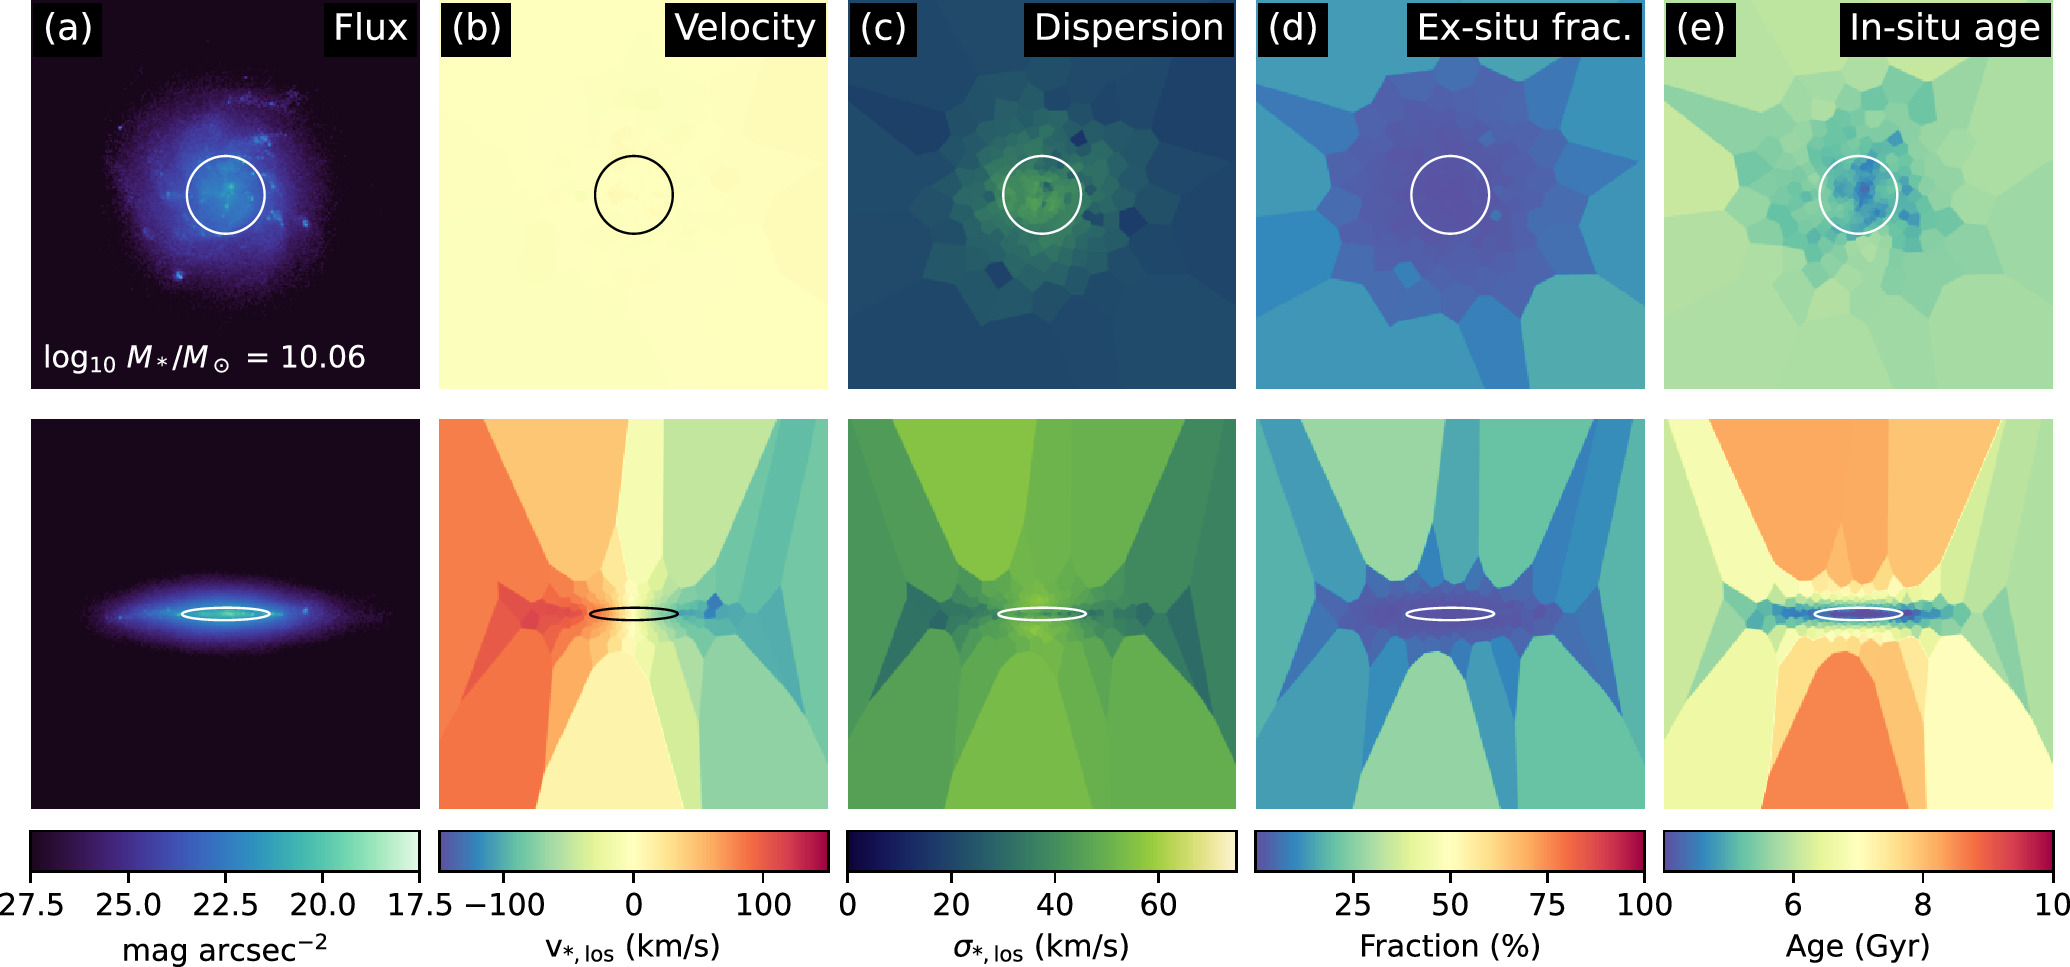
\includegraphics[width=0.75\linewidth]{Han2024.jpg}
    \caption{Figures show face-on and edge-on projections of (a) flux, (b) velocity, (c) dispersion, (d) ex situ fraction, and (e) age of in situ stars. }
    \label{fig:enter-label}
\end{figure}


Based on the work of Stickley et al. (2012) It is suggested by his N-body simulations that the velocity dispersion increases when a galaxy merger occurs. As figure one shows the final equilibrium of the velocity dispersion increases from the value at $t=0$. I predict that this is happening because of the addition of mass and energy into a system. Similarly to a person sitting in a chair if you give them extra weights or push the chair they are spinning in, their direction and speed are subject to change.

%% For this sample we use BibTeX plus aasjournalv7.bst to generate the
%% the bibliography. The sample7.bib file was populated from ADS. To
%% get the citations to show in the compiled file do the following:
%%
%% pdflatex sample7.tex
%% bibtext sample7
%% pdflatex sample7.tex
%% pdflatex sample7.tex

\bibliography{citations}{}
\bibliographystyle{aasjournalv7}

%% This command is needed to show the entire author+affiliation list when
%% the collaboration and author truncation commands are used.  It has to
%% go at the end of the manuscript.
%\allauthors

%% Include this line if you are using the \added, \replaced, \deleted
%% commands to see a summary list of all changes at the end of the article.
%\listofchanges

\end{document}

% End of file `sample7.tex'.
